\documentclass{article}
\usepackage{multirow}
\usepackage{longtable}
\usepackage{float}
\usepackage{parskip}
\usepackage[margin=0.75in]{geometry}
\usepackage{pgfplots}
\usepackage{graphicx}
\pgfplotsset{compat=1.18}
\title{Assignment 3}
\author{Garvit Shah [U21CS089]}
\date{February 2023}
\begin{document}
   \maketitle

   \section*{Hardware Details}
   \begin{itemize}
    \item Memory: 8 GB 1600 MHz DDR3
    \item Processor: 1.8 GHz Dual-Core Intel Core i5
  \end{itemize}

  \section*{Software Details}
  \begin{itemize}
   \item Apple clang version 14.0.0 clang-1400.0.29.202
   \item xcode-select version 2395.
  \end{itemize}

   \section{2-Way Merge Sort}
   \subsection{Algorithm}
   \begin{enumerate}
    \item Create a file pointer and Open the File
    \item Read the number from the file and put it in an array.
    \item Divide the array into two equal parts recursively till you are left with one element.
    \item After reaching the base case, call merge function.
    \item Merge Funciton merges two divided arrays.
   \end{enumerate}
   
   \subsection{Observations}
   \begin{table}[h!] 
   \centering     
   \begin{tabular}{ | p{3cm} | p{3cm} | p{3cm} | }  
    \hline
    \multicolumn{3}{|c|}{Time Complexity for 2-way Merge Sort} \\
    \hline
    File Name & No. of Entries & Average Case\\
    \hline 
    File-1 & 1024 & 0.00379398 \\
    File-2 & 4096 & 0.0158169 \\ 
    File-3 & 16384 & 0.0653478 \\ 
    File-4 & 65536 & 0.271358 \\ 
    File-5 & 262144 & 1.13362 \\ 
    File-6 & 1048576 & 5.25466 \\ 
    File-7 & 2097152 & 10.6776 \\ 
    File-8 & 4194304 & 21.6901 \\ 
    File-9 & 8388608 & 44.4687 \\
    File-10 & 16777216 & 72.4756 \\  [1ex]
    \hline
   \end{tabular}
   \caption{Time taken for 2-way Merge Sort}
\end{table}

\section{3-Way Merge Sort}
\subsection{Algorithm}
\begin{enumerate}
 \item Create a file pointer and Open the File
 \item Read the number from the file and put it in an array.
 \item Divide the array into three equal parts recursively till you are left with one element in each divided array.
 \item After reaching the base case, call merge function.
 \item Merge Funciton merges three divided arrays.
\end{enumerate}

\subsection{Observations}
\begin{table}[h!] 
\centering     
\begin{tabular}{ | p{3cm} | p{3cm} | p{3cm} | }  
 \hline
 \multicolumn{3}{|c|}{Time Complexity for 3-way Merge Sort} \\
 \hline
 File Name & No. of Entries & Average Case\\
 \hline 
 File-1 & 1024 & 0.00379398 \\
 File-2 & 4096 & 0.0158169 \\ 
 File-3 & 16384 & 0.0653478 \\ 
 File-4 & 65536 & 0.271358 \\ 
 File-5 & 262144 & 1.13362 \\ 
 File-6 & 1048576 & 5.25466 \\ 
 File-7 & 2097152 & 10.6776 \\ 
 File-8 & 4194304 & 21.6901 \\ 
 File-9 & 8388608 & 44.4687 \\
 File-10 & 16777216 & 72.4756 \\  [1ex]
 \hline
\end{tabular}
\caption{Time taken for 3-way Merge Sort}
\end{table}

\newpage
\subsection{Graph}
\begin{center}
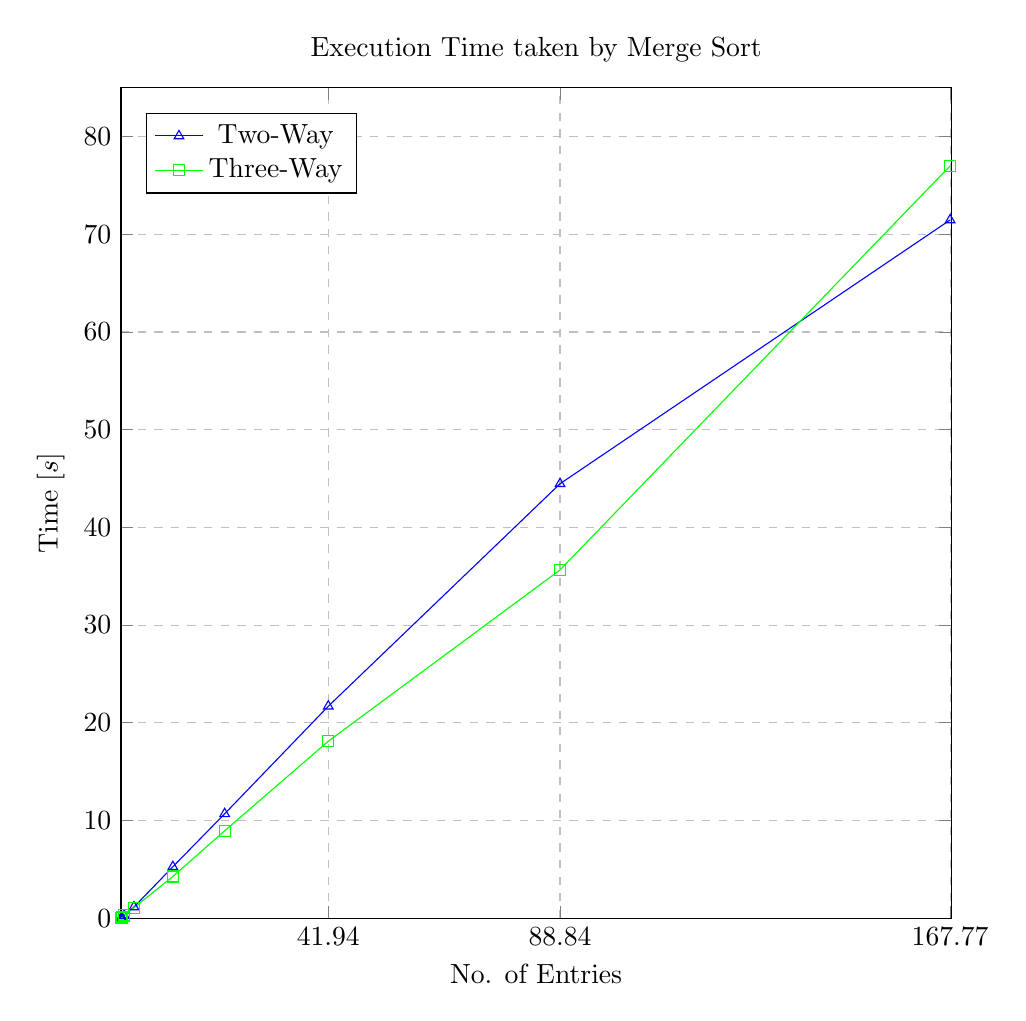
\begin{tikzpicture}
   \begin{axis}[
       title={Execution Time taken by Merge Sort},
       xlabel={No. of Entries},
       ylabel={Time [\(s\)]},
       xmin=0, xmax=168,
       ymin=0, ymax=85,
       xtick={41.94304,88.83608,167.77216},
       ytick={},
       height = \textwidth,
       width = \textwidth,
       legend pos=north west,
       grid = both,
       grid style=dashed,
       legend entries = {Worst Case}
   ]
   \addplot[
       color=blue,
       mark=triangle,
       ]
       coordinates {
       (0.01024,0.00379398)(0.04096,0.0158169)(0.16384,0.0653478)(0.65536,0.271358)(2.62144,1.13362)(10.48576,5.25466)(20.97152,10.6776)(41.94304,21.6901)(88.83608,44.4687)(167.77216,71.4756)
       };
    
    \addplot[
      color=green,
      mark=square,
      ]
      coordinates {
      (0.01024,0.003449)(0.04096,0.014345)(0.16384,0.061138)(0.65536,0.266912)(2.62144,1.05624)(10.48576,4.25805)(20.97152,8.93716)(41.94304,18.1086)(88.83608,35.6444)(167.77216,77.0121)
      }; 
    
    \legend{Two-Way, Three-Way}
   \end{axis}
   \end{tikzpicture}
\end{center}

\subsection{Conclusion}
The graph for the worst case is of type $nlogn$. This type of curve implies that
the change in time taken is linearly and logarithimically dependent on the change in the no. of elements in the file,
as the line is given by $y = xlog(x)$.
Therefore, it can be concluded that the time complexity for Merge Sort is $O(nlog(n))$.
Theoretically also time complexity comes out to be $O(nlog(n))$. Thus the conclusion matches to the theoretical
value of the time complexity.

\textbf{Time Complexity = $\theta(nlog(n))$}
\end{document}